\chapter{Despliegue y pruebas}
\label{chap:despliegue}

\textcolor{red}{En este capítulo describiremos cómo se llevó a acabo el despliegue de la solución y las pruebas que se realizaron.}

\section{Despliegue}

Debido a la gran cantidad de microservicios que componen la solución, desde muy temprano fue necesario definir un plan de despliegue. Su número iba en aumento y era muy complicado gestionarlos a mano. Para ello, optamos entonces por empaquetarlos en contenedores de \texttt{Docker}\footnote{Página oficial: \url{https://www.docker.com/}}. Gracias a esto podíamos iniciarlos y pararlos fácilmente. Además que nos aporta una serie de ventajas interesantes: ejecución aislada de los procesos, gestión más fácil de las dependencias, entre otras. \cite{newmanBuildingMicroservicesDesigning2021,delatorreNETMicroservicesArchitecture2021}

\begin{wrapfigure}{r}{0.23\linewidth}
  \vspace{-25pt}
  \centering
  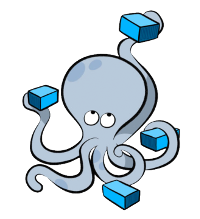
\includegraphics[scale=0.95]{cap_despliegue/images/docker-compose-logo}
  \vspace{-15pt}
\end{wrapfigure}

Para orquestar el despliegue de la solución optamos por \texttt{Docker Compose}\footnote{Página oficial: \url{https://docs.docker.com/compose/}}. Nos permite declarar la configuración del despliegue de nuestros servicios. Esto incluye los parámetros de ejecución, número de instancias, políticas de reinicio, etc. Aunque el bucle MAPE-K \foreign{english}{Lite} original corre sobre Kubernetes, no necesitábamos un orquestador tan ''pesado''. Nuestro plan era ejecutar la solución en un único \foreign{english}{host}.

\texttt{Docker Compose} también nos permite declarar las dependencias entre servicios. Esto fue clave para el despliegue del contenedor de \texttt{RabbitMQ}. Debido a que el protocolo requiere de una conexión permanente al bus\cite{johanssonPartRabbitMQBest2019}, todos los servicios que dependen de él deben desplegarse después. Por ello, declaramos una dependencia con este servicio y definimos una política de reintentos.

\subsection{Observabilidad y telemetría}

Un punto en el que queremos hacer hincapié es en la telemetría. Debido a que estamos tratando con un sistema distribuido, es complicado conocer su estado global en un momento determinado. Especialmente en este caso, en el que participan más de diez microservicios distintos. Si necesitáramos depurar y diagnosticar el comportamiento del sistema, es muy difícil trazar el impacto de una petición.

Por defecto, solo contábamos con los \emph{logs} (registros), que mostramos en la figura \ref{fig:console-logs}. Aparecen intercalados en una única ventana los de todos los servicios y peticiones concurrentes. Aunque nos pueden resultar utilidad, es una aproximación ineficiente. Incluyen demasiada información y es difícil de procesar para una persona. Además que, según aumente la carga de peticiones, aumentará el número de registros y se volverá más difícil de interpretar.

\begin{figure}[h]
  \centering
  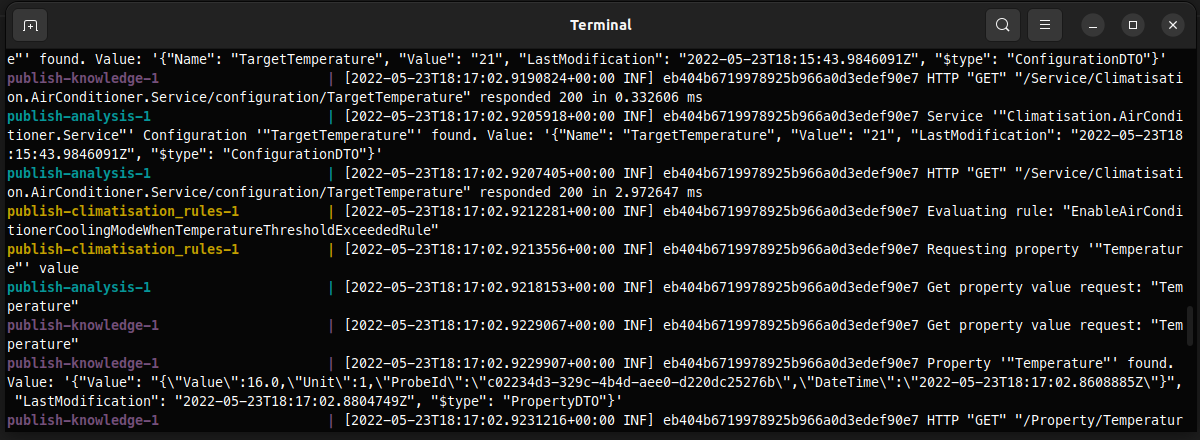
\includegraphics[scale=1.45]{cap_despliegue/images/console-logs}
  \caption{Extracto de \emph{logs} de una ejecución habitual.}
  \label{fig:console-logs}
\end{figure}

En el ámbito de los sistemas distribuidos requerimos de soluciones de monitorización y \foreign{english}{logging} más avanzadas. \cite{newmanBuildingMicroservicesDesigning2021} Nuestros servicios tendrán que recopilar y reportar datos de su funcionamiento, lo que se conoce como \textbf{telemetría}. Esto requerirá de \textbf{instrumentar} nuestros sistemas con distintas herramientas o \textbf{sondas}. Es exactamente lo mismo que hacemos en la etapa de monitorización del bucle MAPE-K.

Para explotar estos datos recurrimos a técnicas de \textbf{observabilidad}. Según \cite{parkerProblemDistributedTracing2020}, la observabilidad <<\emph{no es sólo un método para monitorizar sistemas en producción, si no también para ser capaces de entender su comportamiento usando un número relativamente bajo de señales}>>. Con \textbf{señales} se refiere a las distintas fuentes de información de telemetría de las que dispongamos.

La observabilidad nos ayuda a detectar \textbf{fluctuaciones en el funcionamiento} de nuestro sistema. Estas puedes ser errores, realentizaciones, caídas de servicios, etc. También nos permite \textbf{explicar sus causas} a partir de las señales. De nuestros servicios podemos capturar tres tipos de señales distintos. Todas ellas son complementarias, ya que reflejan el funcionamiento desde distintas perspectivas. Son conocidas como \textbf{los tres pilares de la observabilidad}:

\begin{itemize}
  \item \textbf{\foreign{english}{Logs}}: Se trata de eventos de la aplicación que se registran durante su funcionamiento. Pueden ser simples cadenas de texto o estructuras de datos más complejas. En el segundo caso, se trata de registros enriquecidos con propiedades que les dotan de más contexto. Es el mecanismo de telemetría que ofrece más detalle del funcionamiento de un servicio concreto. También es el más usado.

  \item \textbf{Métricas}: Son datos agregados que nos permiten conocer el estado global de nuestros servicios. \cite{opentelemetryOpenTelemetryDocumentation2022} Se calculan a partir de mediciones de parámetros del servicio en un momento determinado. Por ejemplo del número de peticiones recibidas, su duración, etc. Normalmente se representan cómo series temporales: peticiones por segundo, duración media de las peticiones, etc.

  \item \textbf{Trazas distribuidas}: Se trata del mecanismo más reciente. Es una forma de registrar el recorrido que hace una petición a través de los distintos microservicios que componen nuestro sistema. Nos permite ver cómo participa cada uno de ellos en la operación y qué impacto tiene en el rendimiento. \cite{parkerProblemDistributedTracing2020}

  Para registrar una traza, le asignaremos a la petición un identificador único que se propagará con cada sub-petición. Están compuestas por \foreign{english}{spans}, operaciones que se realizan dentro de la petición. Cada uno puede tener otras sub-operaciones anidadas. \cite{opentelemetryOpenTelemetryDocumentation2022}
\end{itemize}

Para explotar estos datos, necesitaremos entonces poder hacer consultas sobre ellos. Pongamos por ejemplo que hemos detectado que ha aumentado considerablemente la métrica de la duración media de las peticiones. A partir de la fecha y hora de este suceso, deberíamos poder recuperar la información necesaria para responder a la pregunta de qué ha pasado. Ya sean \foreign{english}{logs}, trazas u otras métricas relacionadas.

Con este fin se surgen las \textbf{plataformas de observabilidad}. Se trata de conjuntos de servicios que capturan los datos de telemetría. Los procesan y almacenan para su posterior consulta. También contamos con servicios que nos permiten visualizar y consultar de forma conjunta toda esta información. Por ejemplo, mediante \foreign{english}{dashboards} o paneles.

\subsubsection{Plataforma de observabilidad}

Para poder capturar y explotar estas señales, necesitaremos construir nuestra propia plataforma de observabilidad. Para este trabajo hemos optado por una combinación de cuatro servicios. \texttt{Grafana Loki} para capturar los \foreign{english}{logs}. \texttt{Prometheus} para capturar las métricas. \texttt{Jaeger} para capturar las trazas distribuidas. Y \texttt{Grafana} para visualizar y consultar todos los datos.

\begin{wrapfigure}{r}{0.15\linewidth}
  \vspace{-10pt}
  \hspace{10pt}
  \centering
  
\includegraphics[scale=0.5]{cap_despliegue/images/opentelemetry-logo}
\end{wrapfigure}

Para capturar la telemetría, empleamos el estándar \textbf{OpenTelemetry}\footnote{Página oficial: \url{https://opentelemetry.io/}}. Se trata de un proyecto desarrollado por la Cloud Native Computing Foundation (CNCF). Tiene el objetivo de definir un mecanismo estándar para recopilar y transmitir datos de telemetría. Para ello, ofrece un conjunto de librerias que nos permite instrumentar nuestras aplicaciones. Podremos enviar estos datos a cualquier plataforma que ofrezca extensiones compatibles.

Nuestra plataforma de observabilidad tiene la siguiente estructura (figura \ref{fig:observability-telemetry-collection}):

\begin{figure}[h!]
  \centering
  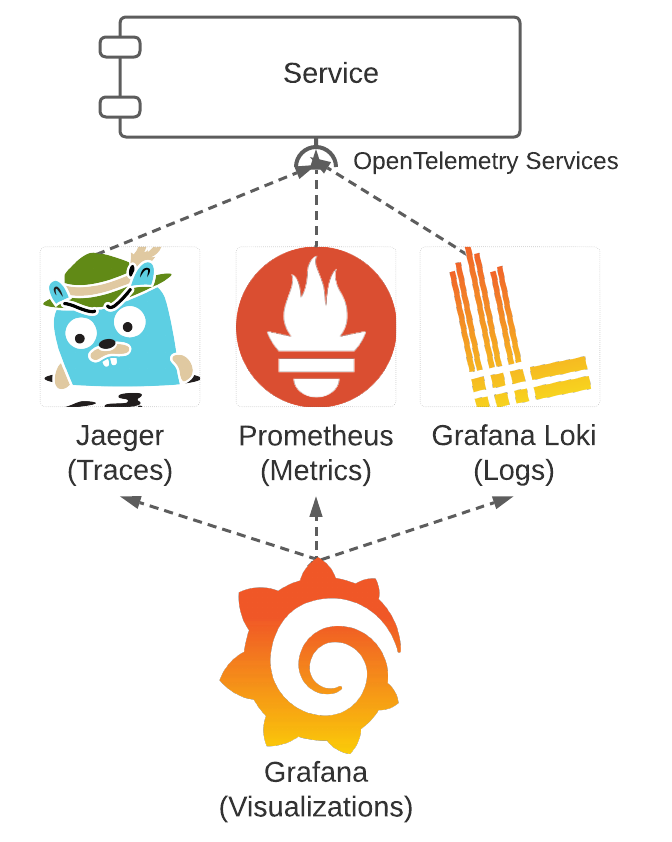
\includegraphics[scale=0.29]{cap_despliegue/images/observability-telemetry-collection}
  \caption{Estructura de nuestra plataforma de observabilidad}
  \label{fig:observability-telemetry-collection}
\end{figure}

\subsubsection{Loki: Logs}
Lo primero que queremos ver es cómo mejorar nuestra estrategia de logging. Lo ideal es añadir identificadores de correlación (el traceID), que nos permita rastrear a través de los distintos servicios una misma traza. Por ejemplo, podemos filtrar a partir de ella para ver todos los detalles de los servicios que intervinieron.

\begin{itemize}
  \item Podemos correlacionar logs de distintos servicios utilizando un identificador único. Por ejemplo, cuando todos surgen a partir de una misma petición. Se trata del \foreign{english}{traceId} (identificador de la traza). \cite{parkerProblemDistributedTracing2020}
\end{itemize}


\subsubsection{Jaeger: Trazas distribuidas}

Gracias a las trazas distribuidas, podemos ver todas las actividades por las que pasó una petición. En nuestro caso, podemos ver por todos los estados por los que paso.

\subsubsection{Prometheus: Métricas}


\subsubsection{Grafana: Visualización}

Desarrollamos un panel de monitorización con Grafana. Esto nos permitía consultar en un solo lugar las métricas, los logs y las trazas.

